\chapter{Background Study}
Ants are social insect. These small tiny creatures have survived major extinction level events in the world. They have been evolved millions of years to survive in the worlds. Their strategies to find resources for their survival are fascinating. We ran several experiments on desert harvester ants at the field to observe how they forage. We have selected three different species of harvester Ants to observe their foraging strategies. Those ants are \textit{P. Rugosus}, \textit{P. Desertorum} and \textit{P. Maricopa}. Our goal was to figure out how they find resources from an environment and what is the effect of the distribution of information on their foraging. So we ran experiments on ants. Seeds in the fields are distributed in a donut shape ring. The area of the food distribution is scaled with the colony size of ants. For example, Desertorum was the smallest in colony size (77$\pm$296), so the donut ring radius of food was 1.5 to 3 meters, Rugosus has a colony size of 1712$\pm$174. So the radius of food distribution for Rugosus was in 5-10 meters. The seeds are organized in a power law distribution around the nest.
\section{\label{section:Power Law}Power Law}
In power law distribution of food, seeds are distributed into multiple piles of different pile size. For example, for power rank 5 of power law distribution total number of seeds will be 1024. And it is divided into 4 types of 256 seeds in each type. One large pile of 256 seeds are placed all together in a certain position. Next 256 seeds are divided into 4 equal sizes of 64 seeds and placed around the nest. Next 256 seeds are equally divided into 16 piles of 16 seeds and placed around the nest inside the ring. Rest of the seeds are distributed uniformly around the nest.
\begin{figure}[h]
	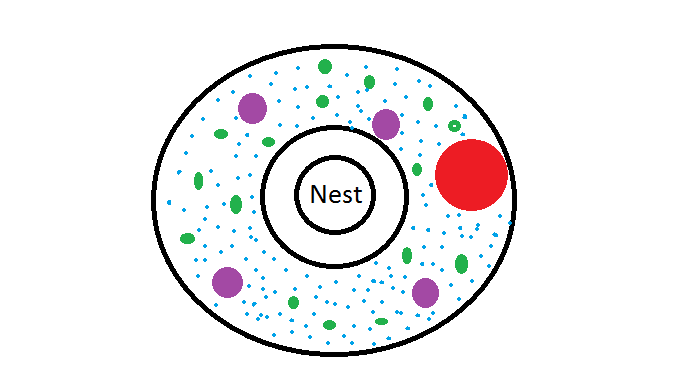
\includegraphics[width=\textwidth]{DonutShape.png}
	\caption{Distribution of Seeds in the field experiment for power law distribution with power rank 5. Red Pile indicates one large pile of 256 seeds. 4 purple piles represent 4 large piles of 64 seeds, Green color represents 16 piles of 16 seeds and blue seeds are 256 random seeds}
\end{figure}
\section{\label{section:CPFA}CPFA}
After the distribution of foods across the nest we observe their collection of seeds. It is observed that ants need longer time to discover the large pile with 256 seeds then the piles with small amount of seeds. But once the seeds are discovered, they started recruiting from the piles. Studies showed that information is transferred among the ants for larger piles with more seeds. We have plotted the collection of seeds from the field experiments and discovered ants walk randomly to collect seeds. Once they get the seed they bring it back to the nest. But if they discover a large food source they share the information with others to recruit from the food source. Once the information is shared more ants come into recruitments and while collecting this food they also share information with other ants. As soon as ants start recruiting from the food source, their foraging rate goes up. But the food source starts losing the number of seeds. As the number of seeds starts decreasing from the food source the recruitment of amount of ants also starts decreasing. Based on this behavior, an algorithm was proposed to simulate the behavior of ants. It is called Central Place Foraging Algorithm(CPFA). CPFA is an agent-based model where agents are programmed to follow ant’s strategy to collect seeds. In CPFA Ants follows three methods to collect seeds. 
